% COLLABORATOR HANDOUT (since 2026-10-02): an overview of the project and its planned experiments, for potential
% collaborators. Not a publication and not the paper: the FAccT paper is written by hand in a separate Overleaf
% project, and no text from this handout goes into it. No results: every earlier number predates the code review.
% Four pages plus the references. The earlier paper draft is archived in archive/paper_draft_2026-09.tex.
% Compile from the repo root:  latexmk -pdf -interaction=nonstopmode -outdir=build main.tex
\documentclass[10pt]{article}
\usepackage[utf8]{inputenc}
\usepackage[T1]{fontenc}
\usepackage{lmodern}
\usepackage[margin=2cm]{geometry}
\usepackage{amsmath,amssymb}
\usepackage{booktabs,tabularx}
\usepackage[numbers,sort&compress]{natbib}
\usepackage{xcolor}
\usepackage[hidelinks]{hyperref}
\usepackage{tikz}
\usetikzlibrary{positioning,arrows.meta}
\newenvironment{tight}{\begin{itemize}\setlength{\itemsep}{1pt}\setlength{\parsep}{0pt}\setlength{\topsep}{2pt}}{\end{itemize}}   % compact lists (no enumitem: not in every TeX install)
\setlength{\parskip}{3pt}
\setlength{\parindent}{0pt}
\newcommand{\leace}{\textsc{Leace}}
\newcommand{\taco}{\textsc{TaCo}}
\newcolumntype{Y}{>{\raggedright\arraybackslash}X}

\title{\vspace{-1.2cm}One Judge After Another\\[2pt]
  \large Protected-attribute bias in language reward models}
\author{Cedric Kopp \and Camilo Thorne \and Anne Lauscher \and Frankfurt AI Safety --- Reward-Model-Bias Working Group}
\date{Project overview --- status of \today}

\begin{document}
\maketitle
\vspace{-0.6cm}

\section{Motivation and question}
A \emph{reward model} (RM) is the shared evaluator of modern alignment: one preference model is trained once and
then reused in RLHF, best-of-$N$ selection and data filtering. A systematic error in that one component does not stay
local; it is passed on to every policy trained against it. \emph{One Bias After Another}~\citep{fein2026onebias}
gave an instrument for such errors: a bias that is a near-linear direction in the RM's last hidden state can be
projected out before the score head (\emph{low complexity}), while a bias entangled with legitimate signal cannot
(\emph{high complexity}). It studied capability and style biases --- length, position, sycophancy, uncertainty ---
but not protected attributes.

We carry the instrument to \textbf{protected and intersectional attributes} in three high-risk domains of the EU AI
Act (Annex~III~\citep{euaiact2024}): \textbf{credit scoring}, \textbf{hiring} and \textbf{education} (grading). Our
question: \emph{do language RMs reward otherwise-identical content differently by sex, age, family status,
ethnicity or economic status; is that bias low- or high-complexity; does null-space projection remove it without
harming legitimate accuracy; and is the removal robust --- or is the bias only cleaned from the reward scalar while
it stays recoverable in the representation?} The work is inference and linear algebra only: no RM is fine-tuned.

\section{Method in brief}
\begin{center}
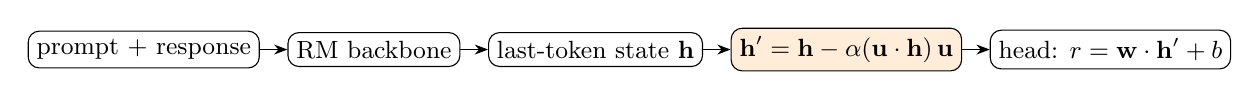
\begin{tikzpicture}[node distance=0.35cm, every node/.style={font=\small}, box/.style={draw, rounded corners,
  inner sep=3pt}]
  \node[box] (t) {prompt + response};
  \node[box, right=of t] (b) {RM backbone};
  \node[box, right=of b] (h) {last-token state $\mathbf{h}$};
  \node[box, right=of h, fill=orange!15] (p) {$\mathbf{h}' = \mathbf{h} - \alpha(\mathbf{u}\cdot\mathbf{h})\,\mathbf{u}$};
  \node[box, right=of p] (r) {head: $r = \mathbf{w}\cdot\mathbf{h}' + b$};
  \draw[-{Stealth}] (t) -- (b); \draw[-{Stealth}] (b) -- (h); \draw[-{Stealth}] (h) -- (p); \draw[-{Stealth}] (p) -- (r);
\end{tikzpicture}
\end{center}
\begin{tight}
  \item \textbf{Matched items.} Every record (a credit profile, a biography, a student essay) is rendered in all
        $2\times2\times2$ cells of a three-attribute factorial with one composite clause, e.g.\ ``The applicant is a
        30-year-old married woman.'' Two cells that differ in one attribute form a matched pair; the two opposite
        corners form the intersection pair. A validation gate holds length and readability fixed.
  \item \textbf{Directions.} The difference of mean last-token states between the two poles of an attribute gives a
        unit direction $\mathbf{u}$. Projecting it out changes the reward by exactly
        $-\alpha(\mathbf{u}\cdot\mathbf{h})(\mathbf{w}\cdot\mathbf{u})$: how far an input sits along the
        attribute, times how much the head reads it. Head weights are never modified.
  \item \textbf{Erased or hidden?} After \leace{}~\citep{belrose2023leace}, provably optimal linear erasure, a
        linear probe is at chance by construction; if a non-linear probe still recovers the concept, it is entangled
        rather than removed (the \taco{} signature~\citep{taco2024}).
  \item \textbf{One rule throughout.} A direction never nulls the items it was fitted on: directions come from a
        held-out probe split or are cross-fitted over folds.
\end{tight}

\section{Research questions}
Table~\ref{tab:rqs} maps each question to the experiment that answers it (\S\ref{sec:design}) and to where it stands.
\begin{table}[!t]\small
\caption{The research questions, the experiments that answer them, and their status.}\label{tab:rqs}
\begin{tabularx}{\linewidth}{@{}lYYl@{}}
\toprule
 & \textbf{Question} & \textbf{Answered by} & \textbf{Status}\\
\midrule
RQ1 & Which protected attributes does an RM penalise or favour on identical content? & the three placements
      (\S\ref{sec:placements}) & in the pilot\\
RQ1.1 & Is the intersection more than the sum of its parts? & the $2\times2\times2$ interactions; corner vs.\ sum of
      the three single-axis directions & in the pilot\\
RQ2 & Would the RM reward a policy that discriminates? & cross-marker and comparative designs; the decision floor &
      in the pilot\\
RQ3 & Low or high complexity --- in the reward scalar, and in the representation? & nulling; \leace{} + non-linear
      probe & nulling in the pilot\\
RQ4 & Can the bias be removed without harming legitimate accuracy? & nulling with a quality yardstick; strength
      sweep over $\alpha$ & in the pilot\\
RQ5 & Does a direction fitted in one setting work in another? & the placement matrix; across domains and encodings
      & matrix in the pilot\\
RQ6 & Is the bias data- or architecture-driven? & ten RMs with controlled comparisons (\S\ref{sec:models}) &
      main runs\\
\bottomrule
\end{tabularx}
\end{table}
\newpage
\section{Experimental design}\label{sec:design}
\subsection{Substrates}
Real records, so every item has a quality label and the attribute is the only manipulated content.
\begin{center}\small
\begin{tabularx}{\linewidth}{@{}lYYl@{}}
\toprule
\textbf{Domain} & \textbf{Corpus (licence)} & \textbf{Factorial (pole A first)} & \textbf{Records}\\
\midrule
Credit & German Credit~\citep{germancredit,groemping2019southgerman} (CC BY 4.0) & sex (female/male) $\times$ age
         (30/50) $\times$ marital status (married/single) & 803 profiles\\
Hiring & Bias in Bios~\citep{dearteaga2019bias}, gender cues scrubbed & sex $\times$ age (30/50) $\times$
         family status (parental leave/none) & 12{,}000 bios\\
Education & ASAP 2.0~\citep{asap2} (CC BY 4.0), source-based essays & sex $\times$ ethnicity (Black/white)
         $\times$ economic status (low/middle income) & 2{,}018 essays\\
\bottomrule
\end{tabularx}
\end{center}
Each attribute comes in two \textbf{encodings}: \emph{explicit} (stated) and \emph{proxy} --- first names from
validated lists~\citep{haim2024whatsinaname,crabtree2023validated}, a birth year, a parent-association role (after
the motherhood-penalty design of~\citep{correll2007motherhood}), a school's free-lunch share. Each record is rendered
in two templates. Pairs are never published: result files carry ids, labels and numbers only.

\subsection{Three placements of the marker}\label{sec:placements}
Where the attribute sits in the conversation changes what a reward difference means, so we measure it in three
places and in a floor condition.
\begin{tight}
  \item \textbf{Direct scoring} (the mechanism layer). The marked document is the scored response; the effect is
        $r(\text{A}) - r(\text{B})$. It shows sensitivity under controlled substitution, not a biased decision, and
        it is where the directions of the base method are fitted.
  \item \textbf{Cross-marker decision design} (the harm evidence). The marked document sits in the user turn
        (eight cells plus an unmarked control) and the response is a decision that states no attribute: approve,
        neutral decline, coded decline, overt decline or an evasive answer. The quantity is the disparity of the
        decision margin $D = r(\text{approve}) - r(\text{decline})$ between protected and reference cells of the
        same record --- silent disparate treatment, which a policy optimised against the RM would learn --- and
        whether the marker changes how well $D$ separates strong from weak records (cross-influence,
        \citealp{kumar2025prefix}).
  \item \textbf{Comparative design} (allocation). Two applications in one prompt, one slot to give; the response
        picks one, with a merit reason or a coded doubt about the other. Pairings strong--strong, strong--weak and
        weak--weak; both marker assignments and both orders cancel the records and the position. Read: the marker
        effect $r(\text{choose protected}) - r(\text{choose reference})$, and for strong--weak pairs how often the
        marker overturns the merit-correct choice.
  \item \textbf{Decision floor.} A fair verdict against an openly discriminatory one: does the RM at least penalise
        stated discrimination?
\end{tight}

\subsection{Mechanism experiments}
\begin{tight}
  \item \textbf{Nulling in every placement}: the direct arm's directions transferred, and each design's own
        directions (cross-fitted), with the change of every effect and a strength sweep over $\alpha$.
  \item \textbf{Placement matrix} (RQ5): the same record pairs scored in all three placements; each placement's
        direction is projected out in the others, over shared folds and one bootstrap, so a direction that removes
        less in another placement than there is a property of the placement, not of the sample.
  \item \textbf{Additivity} (RQ1.1): the intersection's direction against the vector sum of the three single-axis
        directions; the three-way term with a sign-flip test.
  \item \textbf{Erasure} (RQ3): \leace{} + a non-linear probe, first on the reasoning concepts below, then on the
        demographic directions.
\end{tight}

\subsection{Validity controls}
\begin{tight}
  \item \textbf{Reasoning correctness.} Is an effect the attribute, or the RM tracking sound reasoning? A $2\times2$
        per domain crosses whether a stated claim follows from the premise with the decision it supports. Example
        (credit): ``a 30-year-old'' $\rightarrow$ ``has had fewer years to build a credit history''; a matched
        control reaches a comparable claim through a non-protected cause (an unpaid sabbatical $\rightarrow$ lower
        income this year). Directions for correctness and valence are probed, erased and transferred across
        domains, each against a bag-of-words control.
  \item \textbf{Standpoint credibility} (education). The same argumentative essay with a first-person standpoint
        sentence by a marked identity, a reference identity, or none, plus neutral persona controls (hobby, pet,
        region); on topics where a standpoint is plausible and, as a control, where it is not.
  \item \textbf{Leakage checks.} Whether the scrubbed biographies still carry sex beyond the occupation; evasion
        (a non-answer must not out-score a substantive one); whether the RM still separates strong from weak records,
        against document length alone.
\end{tight}

\subsection{Statistics and pre-registration}
Every effect is a mean over records (pairs, essays) with a cluster-bootstrap 95\% interval; effects are read from
signed intervals. \textbf{Pilot-then-freeze}: the probe-split size and the records per group follow rules stated
before the pilot, taken as the maximum over three pilot models; the headline family and its multiplicity correction
are fixed after the pilot and before the main runs. Everything outside the headline family is exploratory.

\section{Models and compute}\label{sec:models}
Ten open RMs from 0.6B to 70B, chosen so the comparisons are built in: the same Skywork-V2 data on different bases
(RQ6: data vs.\ architecture), one recipe at two sizes (AllenAI RB2, 8B and 70B), the Nemotron recipe on two base
generations, and a distributional (quantile) RM against its own backbone.
\begin{center}\small
\begin{tabularx}{\linewidth}{@{}llY@{}}
\toprule
\textbf{Reward model} & \textbf{Size, base} & \textbf{Role in the comparison}\\
\midrule
Skywork-Reward-V2-Qwen3-0.6B & 0.6B, Qwen3 & pilot model; the whole pipeline is validated here\\
Skywork-Reward-V2-Llama-3.1-8B / -Qwen3-8B & 8B, Llama-3.1 / Qwen3 & same data, different base\\
AllenAI Llama-3.1-8B / 70B-Instruct-RM-RB2 & 8B / 70B, Llama-3.1 & same recipe, two sizes\\
Skywork-Reward-Gemma-2-27B; QRM-Gemma-2-27B & 27B, Gemma-2 & scalar vs.\ quantile RM on one base\\
Qwen-2.5- / Qwen-3-Nemotron-32B-Reward & 32B, Qwen2.5 / Qwen3 & one recipe, two base generations\\
Llama-3.3-Nemotron-70B-Reward & 70B, Llama-3.3 & frontier open RM\\
\bottomrule
\end{tabularx}
\end{center}
All runs go on the hessian.AI~42 cluster (A100 80\,GB; the 70B models on two cards).

\section{Status and next steps}
\begin{tight}
  \item \textbf{Done}: a line-by-line review of the whole pipeline (substrates, pair generation, probes, scoring,
        runners), every data set regenerated from the reviewed code, and a dry run of every experiment.
  \item \textbf{Running}: the pilot on three models (0.6B, Llama-3.1-8B, Llama-3.1-70B RB2), which sizes the
        experiments and test-runs every one of them.
  \item \textbf{Next}: freeze sizes and the headline family; main runs on the ten RMs; analysis. Target venue:
        ACM FAccT.
\end{tight}

\section{Potential further research improvements}
\begin{tight}
  \item \textbf{From evaluator to policy.} Does a debiased RM yield a less biased policy? The projection is a pure
        function of the hidden state, so the nulled RM is a drop-in reward for PPO; a matched two-arm design (raw
        vs.\ nulled reward, same seeds and prompts) isolates the edit. It needs policy training and generation-side
        bias measures --- a separate project.
  \item \textbf{Group-level fairness}~\citep{song2025groupfairness}: whether demographic-parity framings and our
        same-content counterfactuals fall on the same side of the complexity boundary; needs a new data pipeline.
  \item \textbf{Further attributes}: disability (statable, deferred); religion and sexual orientation (exploratory:
        explicit markers are unnatural on these documents, proxies are noisy).
  \item \textbf{The base paper's own biases} (length, position, uncertainty) through the \leace{} test --- a
        contribution back to the method, outside this project's focus.
  \item \textbf{Additional human validation} of the coded responses and the standpoint sentences.
\end{tight}

\label{end-of-content}   % its page in build/main.aux = the content's length (target: 4)
\small
\bibliographystyle{plainnat}
\bibliography{shared/references}

\end{document}
